\documentclass{article}
\usepackage{graphicx}
\graphicspath{ {./images/} }
\usepackage[export]{adjustbox}
\usepackage{amsmath}


\title{13. Polinomi. Gredzeni.}
\author{Gunārs Ābeltiņš}
\date{2022-05-20}

\begin{document}

\maketitle

\section*{1. Uzdevums}
Uzbūvējiet polinomu P(x), kas pieņem šādas vērtības: P(-3)=2; P(-1)=-2; P(0)=1; P(1)=-1; P(3)=1. Vienādojumu sistēmu atrisiniet ar WA. Vai atradīsiet, kā uzzīmēt iegūtā polinoma grafiku?

\begin{equation*}
    P(x) = a_4 x^4 + a_3 x^3 + a_2 x^2 + a_1 x + a_0
\end{equation*}

\begin{equation*}
    P(-3) = a_4 (-3)^4 + a_3 (-3)^3 + a_2 (-3)^2 + a_1 (-3) + a_0 = 2
\end{equation*}
\begin{equation*}
    P(-1) = a_4 (-1)^4 + a_3 (-1)^3 + a_2 (-1)^2 + a_1 (-1) + a_0 = -2
\end{equation*}
\begin{equation*}
    P(0) = a_4 (0)^4 + a_3 (0)^3 + a_2 (0)^2 + a_1 (0) + a_0 = 1
\end{equation*}
\begin{equation*}
    P(1) = a_4 (1)^4 + a_3 (1)^3 + a_2 (1)^2 + a_1 (1) + a_0 = -1
\end{equation*}
\begin{equation*}
    P(3) = a_4 (3)^4 + a_3 (3)^3 + a_2 (3)^2 + a_1 (3) + a_0 = 1
\end{equation*}

\begin{equation*}
    \begin{cases}
        81a_4 - 27a_3 + 9a_2 - 3a_1 + a_0 = 2 \\
        a_4 - a_3 + a_2 - a_1 + a_0 = -2 \\
        a_0 = 1 \\
        a_4 + a_3 + a_2 + a_1 + a_0 = -1 \\
        81a_4 + 27a_3 + 9a_2 + 3a_1 + a_0 = 1
    \end{cases}
\end{equation*}

\begin{equation*}
    P(x) = \frac{23}{72} x^4 - \frac{1}{12} x^3 - \frac{203}{72} x^2 + \frac{7}{12} x + 1
\end{equation*}
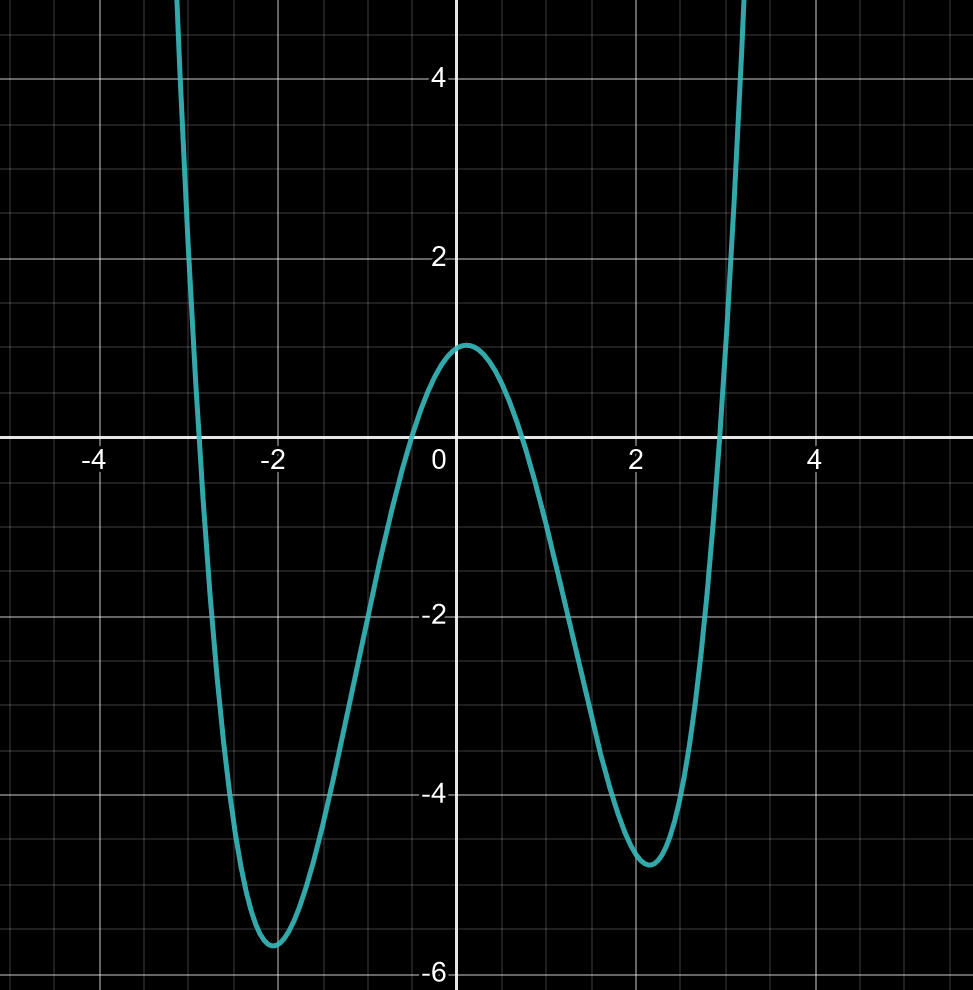
\includegraphics[width=0.9\textwidth, center]{1}

\section*{2. Uzdevums}
Izmantojot tikai gredzena aksiomas un jau iepriekš pierādītās teorēmas, pierādiet T6. Pamatojiet katru secinājumu soli.

\section*{3. Uzdevums}
Izmantojot tikai gredzena aksiomas un jau iepriekš pierādītās teorēmas, pierādiet T6. Pamatojiet katru secinājumu soli.


\end{document}